\chapter{Test Journal: Transmitter integration}\label{appendix:TransmitterInt}
\begin{table}[!h]
\begin{tabular}{l l}
\textbf{Test participants:} & Robin \& Bang\\
\textbf{Date:}  & 02/12-2016
\end{tabular}
\end{table}

\section*{Purpose}
The purpose of this test is to measure how much the amplifier is amplifying the output of the oscillator, which has to be amplified at least \SI{11,02}{\deci\bel} to have an acceptable \gls{snr}, as calculated in \autoref{sec:transmissionPower}. 

\section*{Test equipment and components}
The test equipment and components are listed in \autoref{tab_appendix:Transmitter}.
\begin{table}[!h]
	\centering
	\caption{List of measurement equipment and components}\label{tab_appendix:Transmitter}

	\begin{tabularx}{\textwidth}{lXXXX}
		Name 				& Brand	& Model & AAU-number\\ \toprule \rowcolor{lightGrey}
		Device under test & N/A & N/A & N/A \\
		Signal analyzer & Rohde and Schwarz & Signal Analyser FSIQ 26 & 52766\\
	\end{tabularx}
\end{table}

\section*{Setup}
Diagrams of the setups for measuring the transmitter can be seen on Figures \ref{Appendix:fig:TransmitterSetup} and \ref{Appendix:fig:TransmitterAMP}.
\begin{figure} [!h]
    \centering
        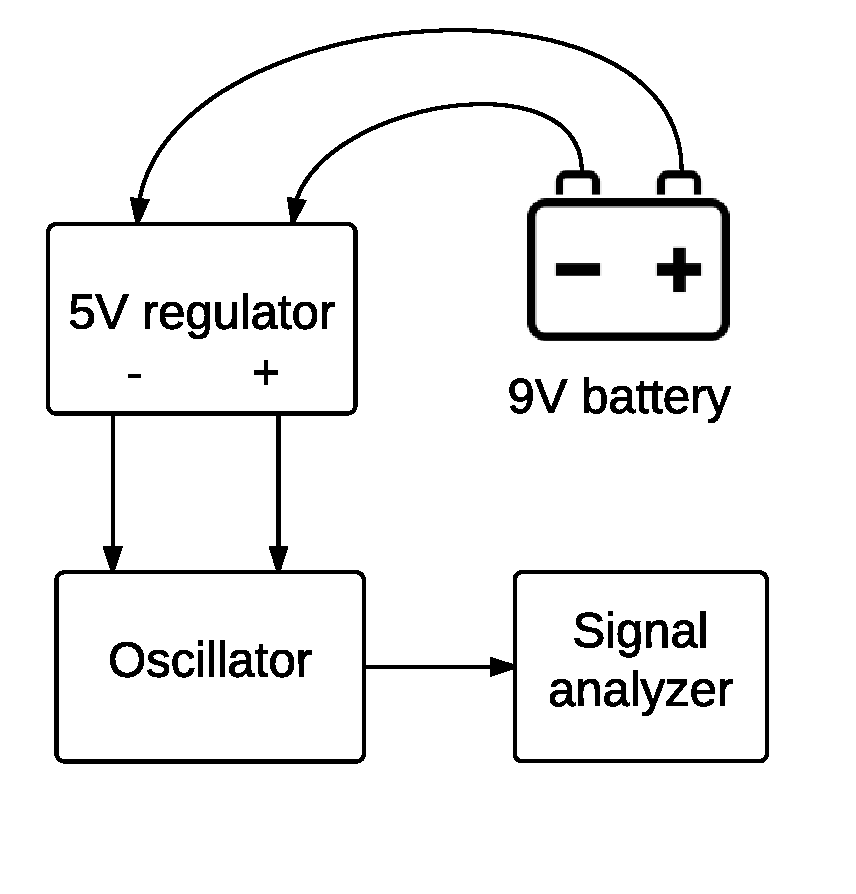
\includegraphics[width=0.5\textwidth]{figures/test/TransmitterOSC}
        \caption{Diagram of the setup for measuring oscillator without amplification.}
        \label{Appendix:fig:TransmitterSetup}
\end{figure}
\begin{figure} [!h]
    \centering
        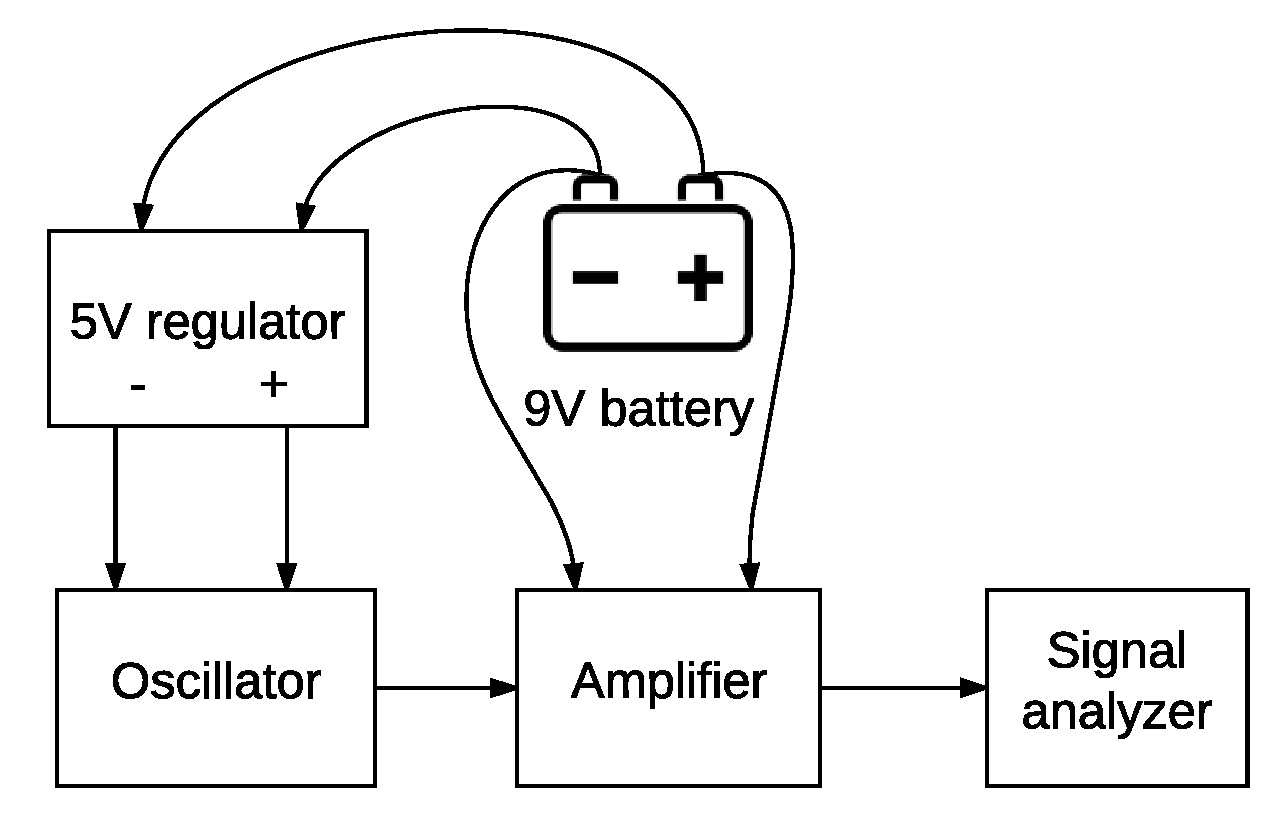
\includegraphics[width=0.6\textwidth]{figures/test/TransmitterAMP}
        \caption{Diagram of the setup for measuring oscillator with amplifier.}
        \label{Appendix:fig:TransmitterAMP}
\end{figure}

\section*{Method}
The first setup of the measurement is without the amplifier connected as seen on \autoref{Appendix:fig:TransmitterSetup}.
The second setup of the measurement is with the amplifier connected as seen on \autoref{Appendix:fig:TransmitterAMP}.

\begin{enumerate}
\item Connect the first setup.
\item Set the potentiometer so the frequency of the oscillator is set to \SI{869}{\mega\hertz}.
\item Measure the received power on the signal analyzer.
\item Connect the second setup.
\item (It might be needed to set the frequency again is the oscillator have drifted)
\item Measure the received power after the amplifier on the signal analyzer.
\end{enumerate}

\section*{Results}
The result of the measurements can be seen on \autoref{Appendix:fig:TransSet1} and \autoref{Appendix:fig:TransSet2}, the data from the figures are also seen in \autoref{tab_appendix:TransmitterResults},.
\begin{figure} [!h]
    \centering
        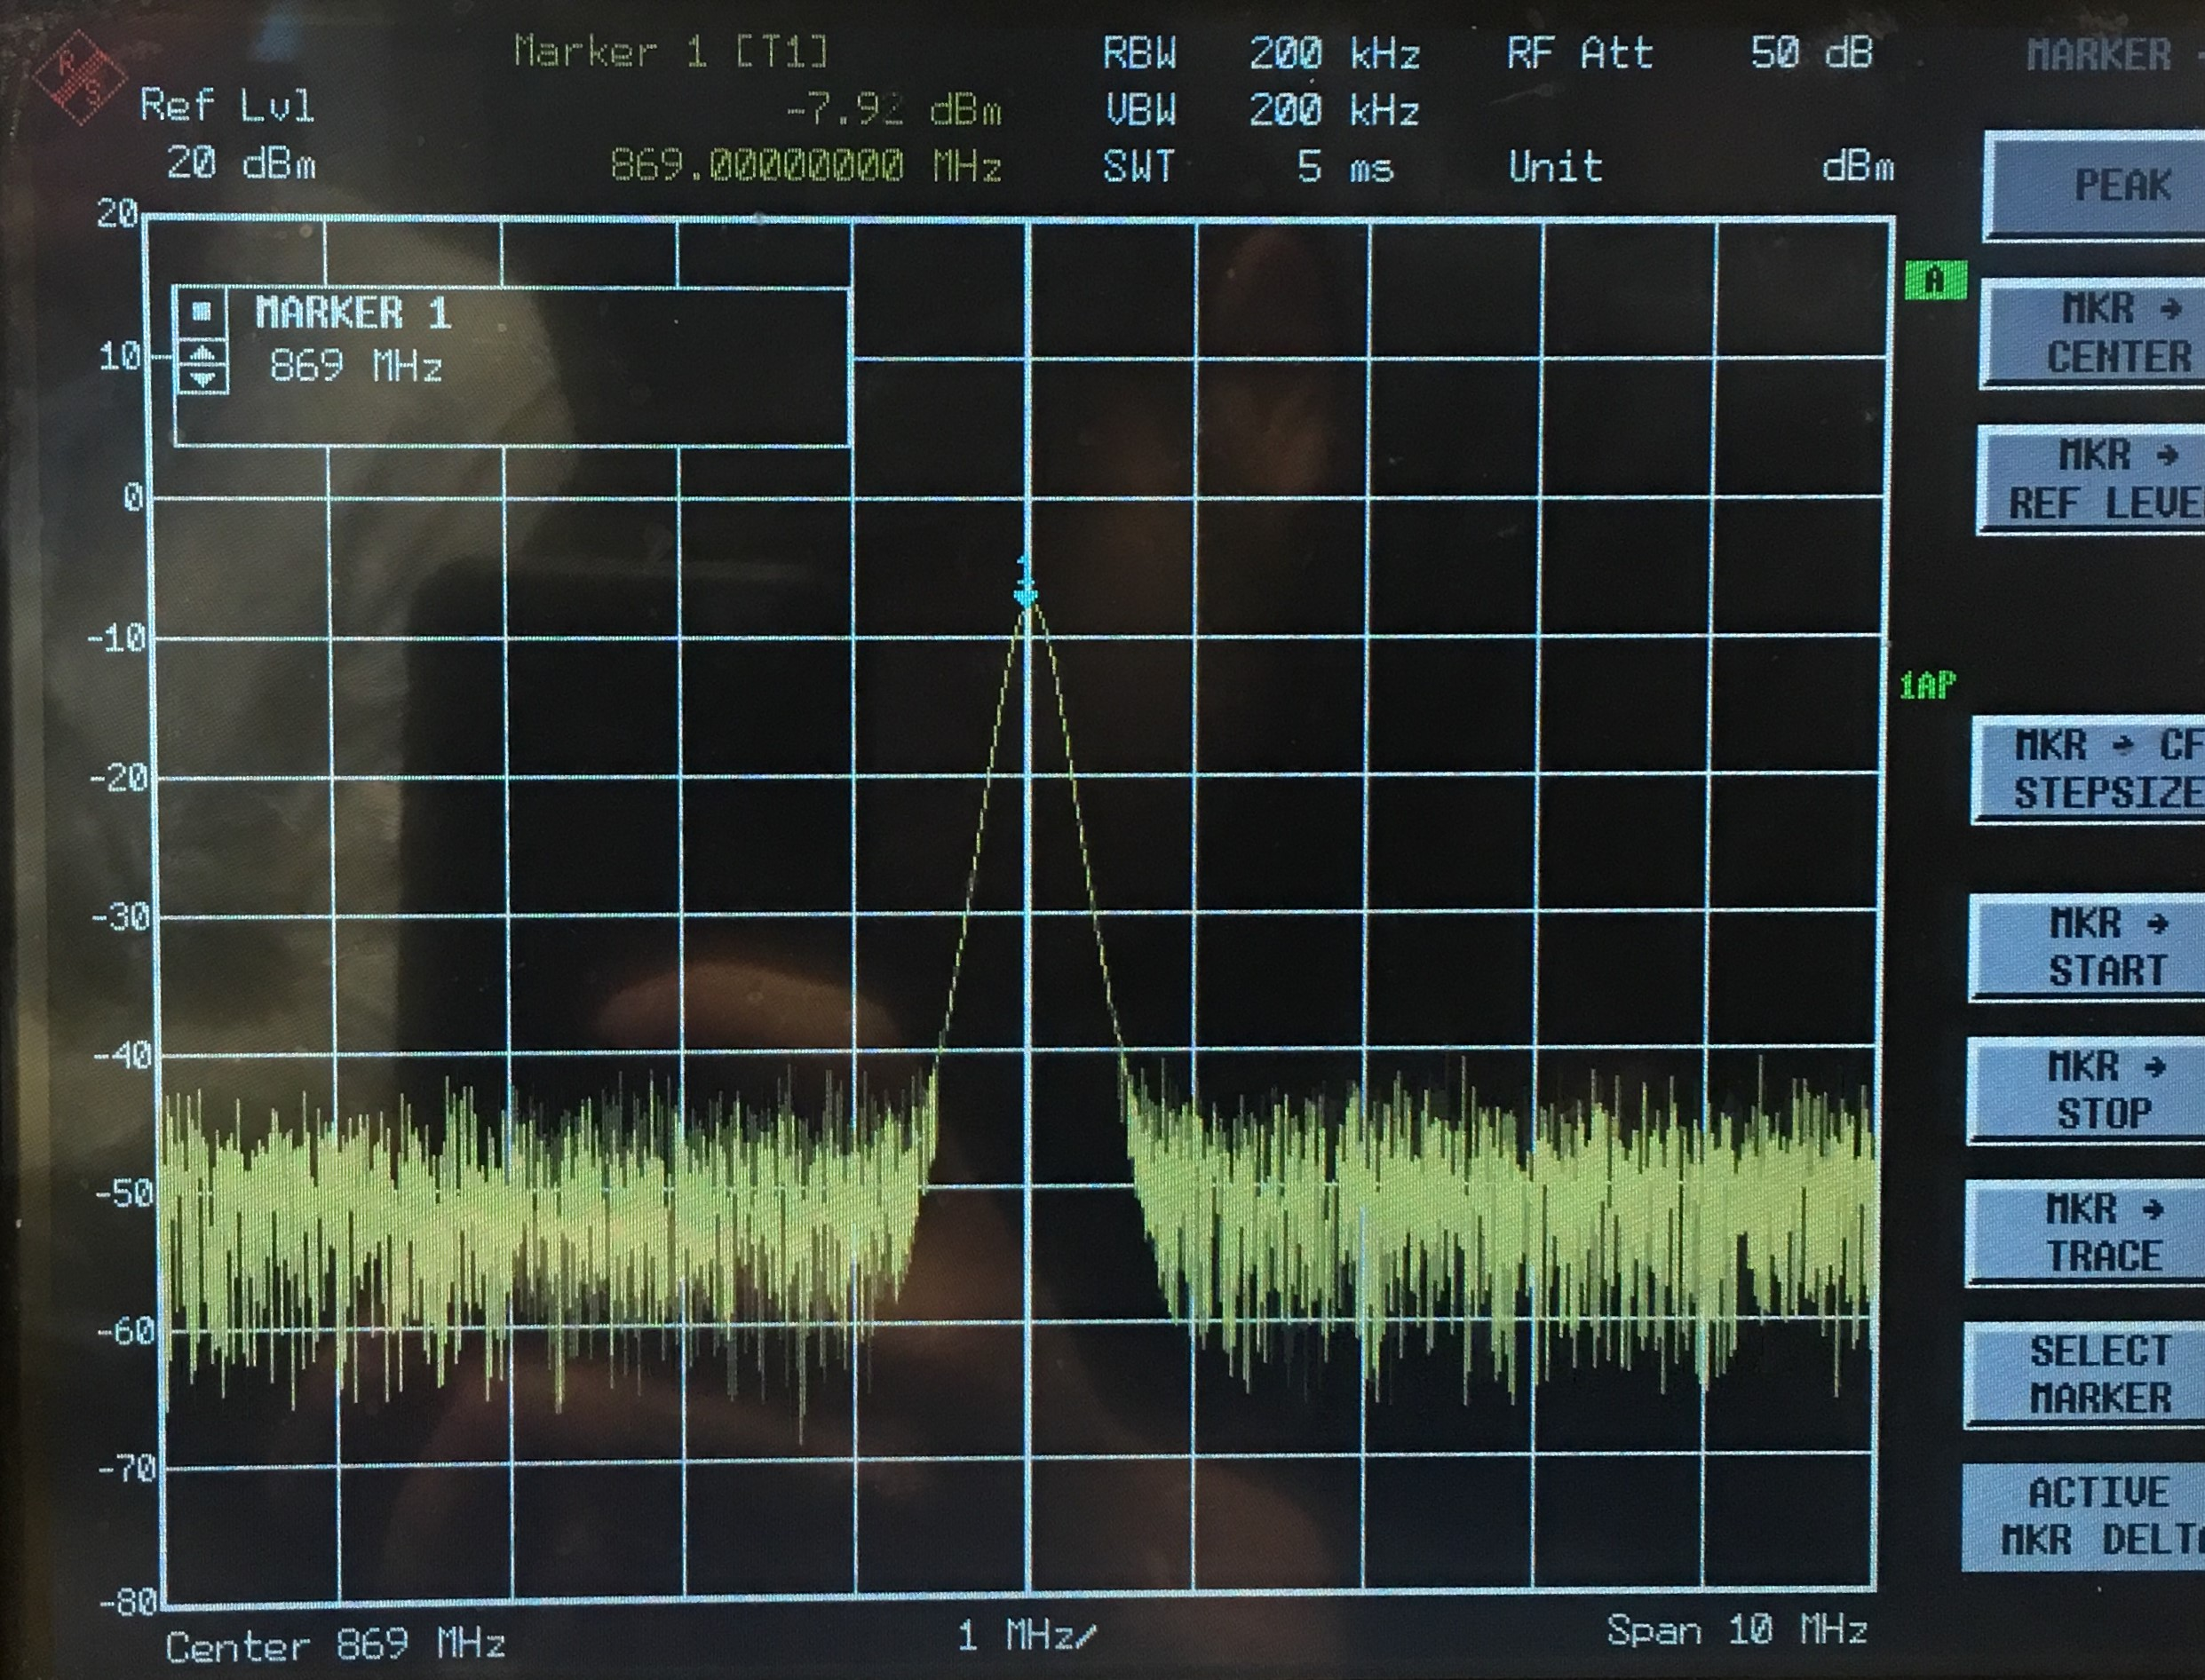
\includegraphics[width=0.5\textwidth]{figures/test/transet1}
        \caption{Measurement without the amplifier.}
        \label{Appendix:fig:TransSet1}
\end{figure}
\begin{figure} [!h]
    \centering
        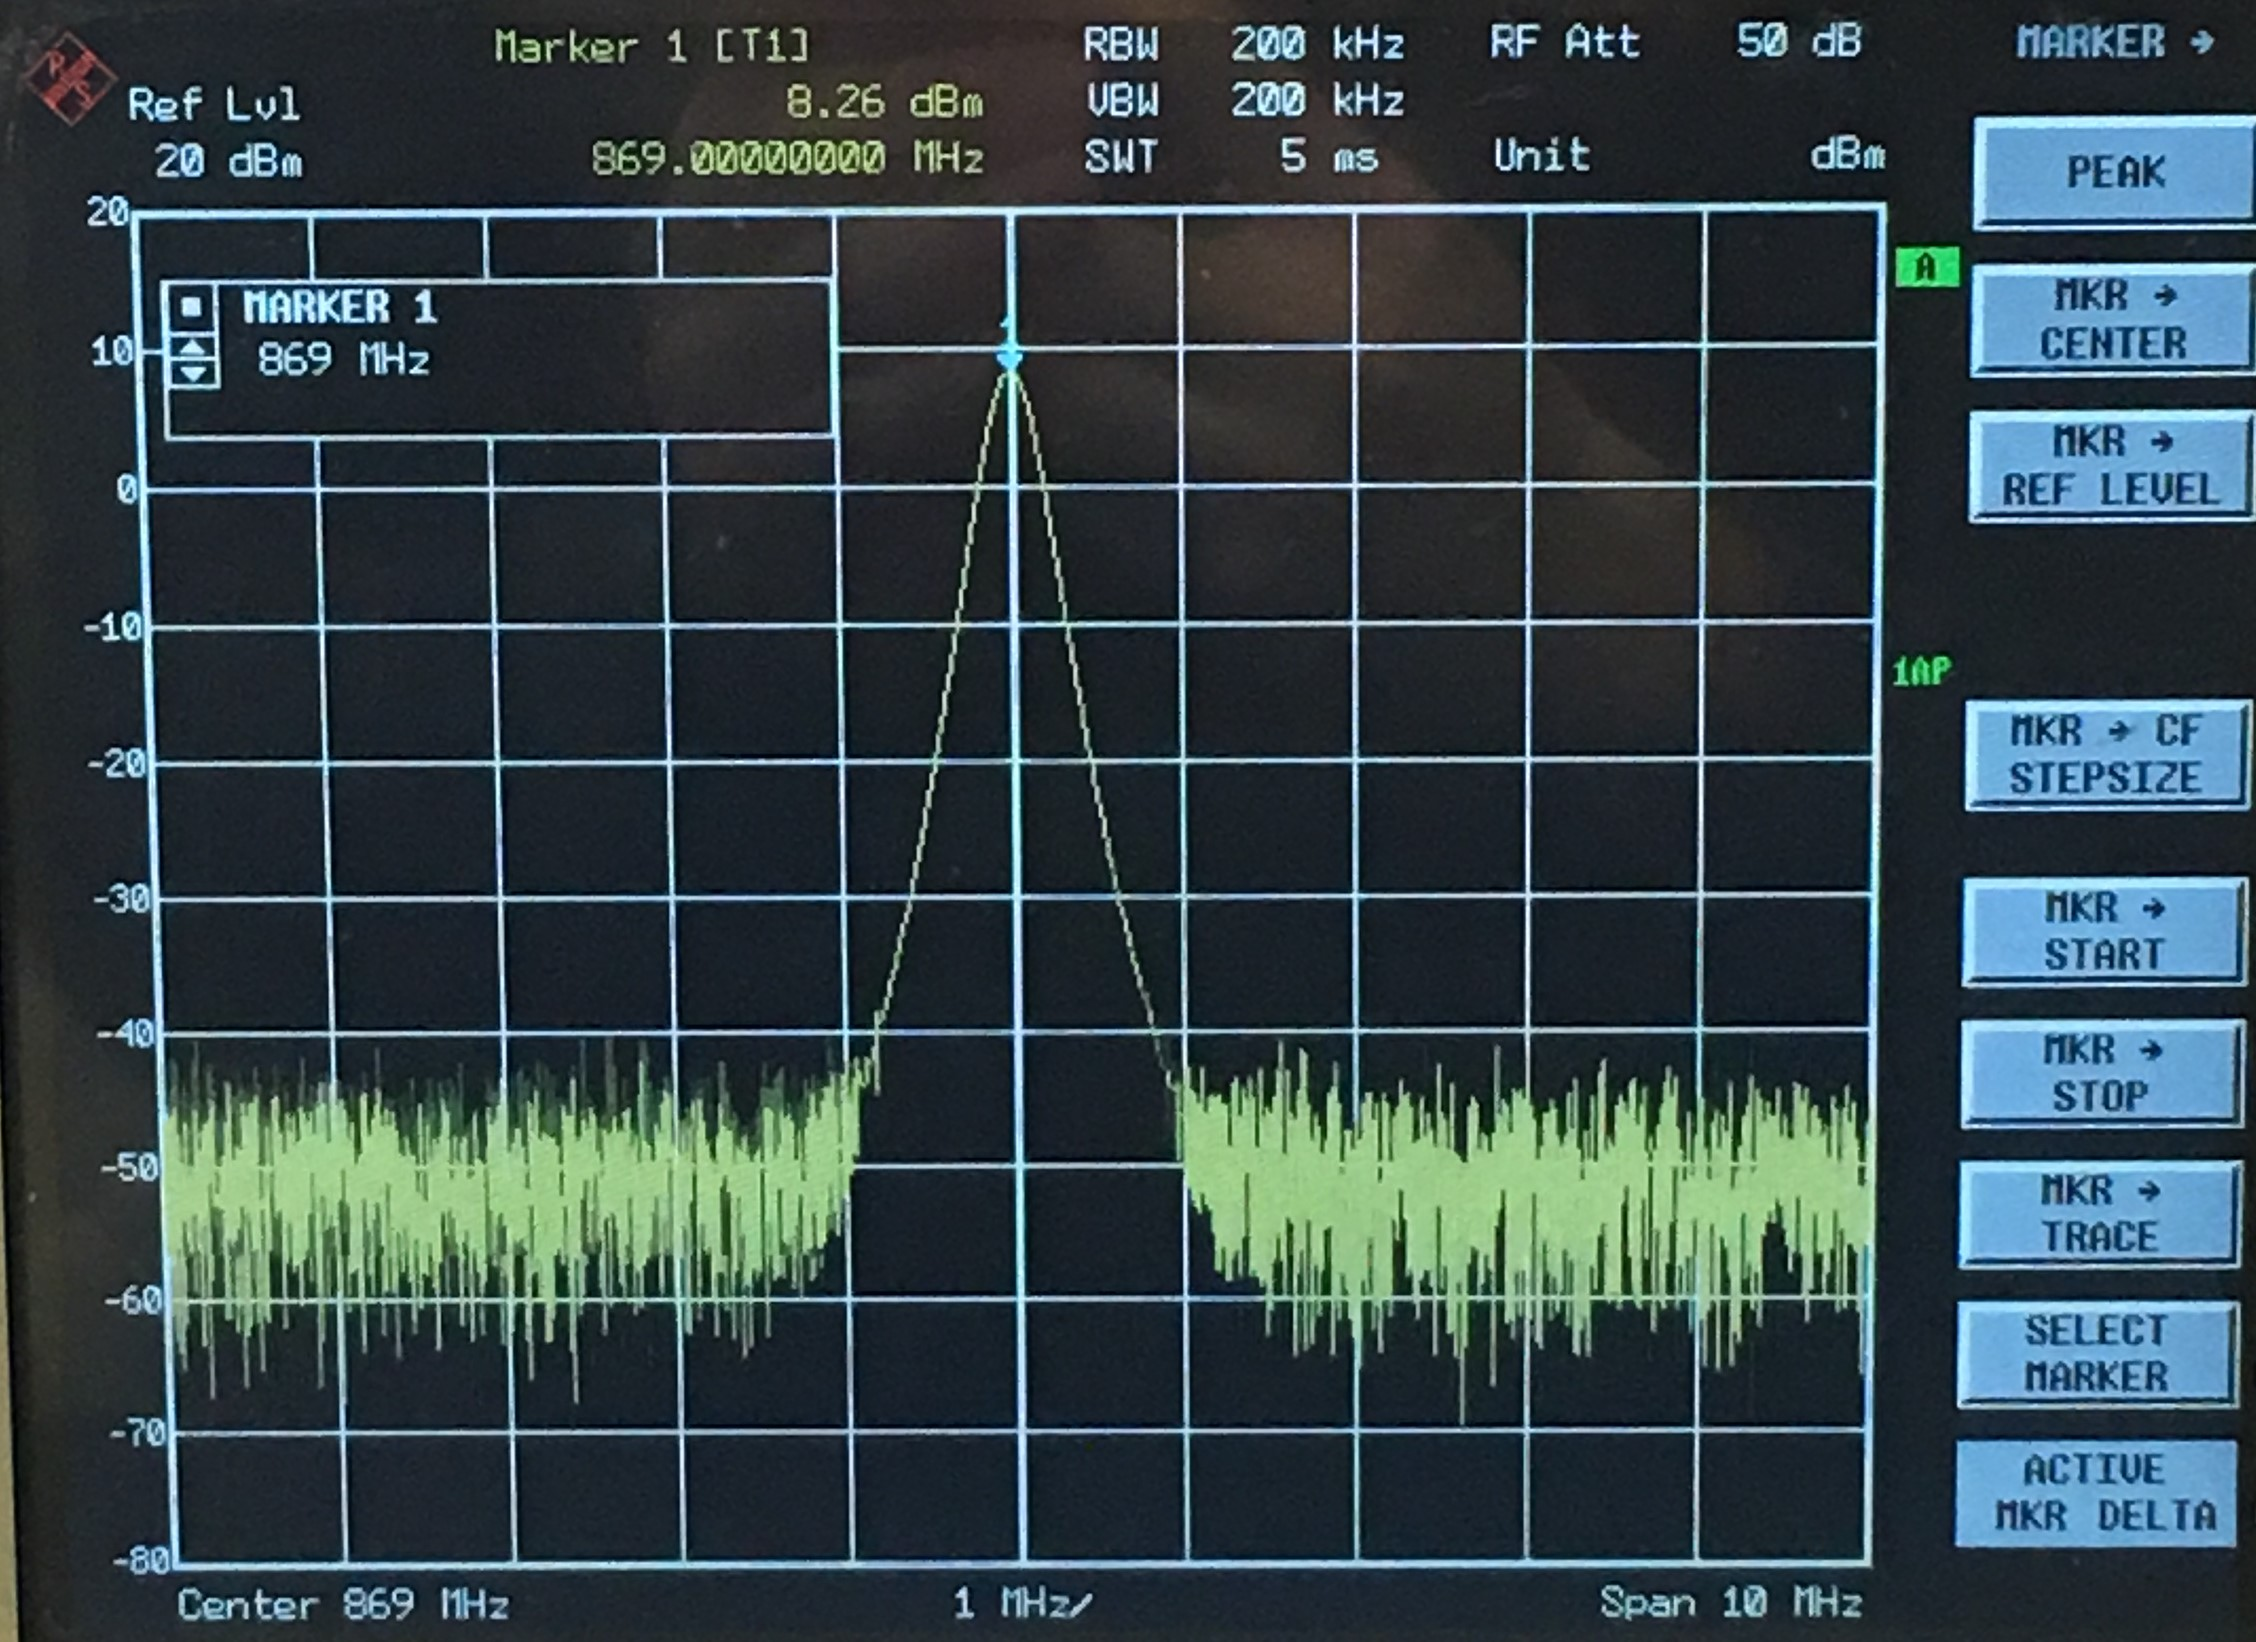
\includegraphics[width=0.5\textwidth]{figures/test/transet2}
        \caption{Measurement with the amplifier.}
        \label{Appendix:fig:TransSet2}
\end{figure}

\begin{table}[!h]
	\centering
	\caption{Data of the measurements.}\label{tab_appendix:TransmitterResults}
	\begin{tabularx}{\textwidth}{lX}
	 Setup & Received power, $P_r$ [\si{\deci\belm}] \\ \toprule \rowcolor{lightGrey}
		1 (Without amplifier) & \SI{-7.92}{\deci\belm} 	\\
		2 (With amplifier)	& \SI{8.26}{\deci\belm} \\ 
	\end{tabularx}
\end{table}

\section*{Data processing}
The result of the measurements show that the amplifier is amplifying the signal \SI{8.26}{}$ - $(\SI{-7.92}{}) =\SI{16.18}{\deci\bel}.

\section*{Conclusion}
The amplifiers amplifies \SI{16.18}{\deci\bel}, which is \SI{5.16}{\deci\belm} more than the minimum \SI{11.02}{\deci\bel} as specified in \autoref{sec:transmissionPower}. It is therefore concluded that the amplifier has sufficient gain.
